\subsubsection{Mecanismo de interacción }

Una parte de la energía de una partícula incidente durante su paso por la materia es directamente proporcional con los daños permanentes o transitorios. Esta cantidad de energía perdida, llamada ``pouvoir d'arrêt total'' (poder de frenado), se define ~como ~$\frac{dE}{dX} \frac{MeV}{cm}$  y está compuesta de dos fenómenos principales: la pérdida de energía electrónica y la pérdida de energía nuclear.

La ionización debida a las interacciones entre las partículas incidentes y los electrones de los átomos del medio atravesado, son la causa principal del fenómeno. Las partes electrónicas tienden a  crear pares electrones-agujeros a lo largo del trayecto de la partícula. Este poder de frenado electrónico se llama LET (\textit{Linear Energy Transfer}) ~\cite{4395093}.
	
El segundo fenómeno corresponde a las colisiones entre las partículas y los núcleos provocando la pérdida de energía nuclear. Esta interacción puede conducir a la eyección del núcleo de una red cristalina. La parte de la energía asociada a este tipo de daños es llamado pérdida de energía no ionizante,  \textit{Non Ionising Energy Loss}(NIEL) ~\cite{316523}.

Se puede entonces concluir que el poder de parada total puede describirse como la suma de estas dos partes de energía:

\begin{equation}\label{EQ1}
\frac{dE}{dX}=\left(\frac{dE}{dX}\right)_\text{electron}+\left(\frac{dE}{dX}\right)_\text{nucleo}
\end{equation}

\subsubsection{Efecto de dosis total}

La dosis es la energía por unidad de masa depositada en un material y que se expresa en Gray. Un Gray es equivalente a observación de un Joule por kilogramo de materia.

En general, una gran parte de los efectos de radiación que se pueden observar se  reagrupan en los llamados efectos de dosis total. Estos efectos resultan de la interacción entre partículas y los aislantes de los circuitos integrados. Cuando una partícula atraviesa un material, la energía que se pierde en su trayectoria puede cederse a los electrones del material atravesado, a este efecto se lo suele llamar dosis ionizante. Si los átomos se  desplazan, decimos que la dosis es no ionizante.


\paragraph{Dosis ionizante}\hfill \break
 
Parte de la energía de las partículas incidentes puede cederse a los electrones del material atravesado. Según la naturaleza del material, los electrones pueden traspasar la banda de conducción como también liberar espacios en la banda de valencia ~\cite{1208572}. En el caso del silicio ligeramente dopado, se puede reconocer que la generación de pares electro-agujeros es equivalente a la densidad de los portadores de cargas en equilibrio. Entonces el efecto es transitorio, ya que el efecto se eclipsará. En el caso de un aislante, el efecto es más crítico. Dos mecanismos (figura ~\ref{Efectos}) que afectan los componentes eléctricos son:
\begin{description}
\item[-] Atrapar las cargas en los aislantes  
\item[-] Migración de las cargas hacia las interfaces aislantes/semi-conductoras y creación de un canal permanente.

\end{description}
Esto tiene una gran cantidad de consecuencias: derivada de la tensión umbral, aumento de la corriente de fuga, disminución de la ganancia, variación de la corriente inversa de los diodos y variación de la tensión de ruptura dieléctrica.

\begin{figure}[H]
	\centering
	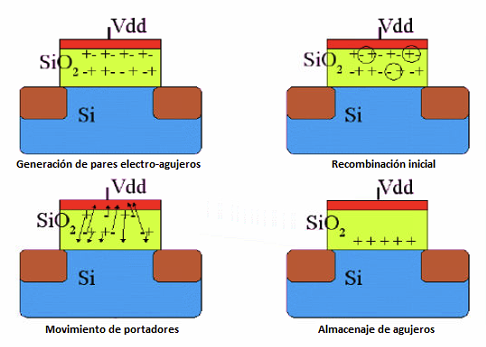
\includegraphics[width=0.8 \textwidth]{img/efectos_cargas.png}
	\caption{Almacenamiento de cargas atrapadas}
	\label{Efectos}
\end{figure}

\paragraph{Dosis no ionizante }\hfill \break

 La introducción de defectos en las redes cristalinas generan nuevas trampas de cargas modificando así las características de funcionamiento del circuito. Como parte de los efectos de dosis ionizantes se pueden citar las siguientes:

\begin{description}
\item[-] Aumento de la corriente de fuga.
\item[-] Modificación del dopaje del semiconductor.
\item[-] Acumulación de cargas atrapadas de los portadores.
\item[-] Efecto túnel
\item[-] Reducción de la vida útil de los portadores minoritarios.
\end{description}


Se debe aclarar que estos efectos afectan los componentes optoelectrónicos como también los transistores bipolares, que son particularmente sensibles a este tipo de daños entre otra series de componentes.